% Nier_ANLP -- SemEval-2026 Task 6 (CLARITY): final presentation (20 min + 10 min questions).
% Same Beamer format as the mid-evaluation deck (report/slides_beamer/main.tex): Madrid theme, navy palette,
% soft frame titles, navy-headed cards, red highlights. Build: bash build.sh -> main.pdf.
% Figures: cd code && python -m figures.slide_figures.   Script and timings: SPEAKER_NOTES.md, STORYBOARD.md.
\documentclass[aspectratio=169,10pt]{beamer}

\usetheme{Madrid}
\usepackage[T1]{fontenc}
\usepackage{lmodern}
\usepackage{graphicx}
\usepackage{booktabs}
\usepackage{array}
\usepackage{amsmath}
\usepackage{pifont}
\usepackage{tikz}
\usetikzlibrary{positioning,arrows.meta,calc,shapes.geometric,fit,backgrounds}

% ---- the mid-evaluation palette and macros, unchanged ----
\definecolor{navy}{RGB}{24,45,86}
\definecolor{accent}{RGB}{176,54,40}
\definecolor{soft}{RGB}{236,240,247}
\setbeamercolor{structure}{fg=navy}
\setbeamercolor{palette primary}{bg=navy,fg=white}
\setbeamercolor{palette secondary}{bg=navy!85!black,fg=white}
\setbeamercolor{palette tertiary}{bg=navy!70!black,fg=white}
\setbeamercolor{title}{bg=navy,fg=white}
\setbeamercolor{frametitle}{bg=soft,fg=navy}
\setbeamercolor{block title}{bg=navy,fg=white}
\setbeamercolor{block body}{bg=soft}
\setbeamertemplate{navigation symbols}{}
\setbeamertemplate{itemize items}[circle]
\setbeamerfont{frametitle}{size=\large,series=\bfseries}
\setbeamerfont{block title}{size=\small,series=\bfseries}
\newcommand{\expsize}{\scriptsize}

\newcommand{\hl}[1]{\textcolor{accent}{\textbf{#1}}}
\newcommand{\takeaway}[1]{\par\vspace{2pt}{\small\textcolor{navy}{\textbf{Takeaway:}} #1}}
\newcommand{\expcard}[4]{%
  \begin{block}{#1}\expsize
    \textcolor{navy}{\textbf{Why:}} #2\\[1pt]
    \textcolor{navy}{\textbf{Result:}} #3\\[1pt]
    \textcolor{navy}{\textbf{Takeaway:}} #4
  \end{block}}
\newcommand{\excard}[4]{%
  \begin{block}{#1}\scriptsize
    \textcolor{navy}{\textbf{Sub-question:}} #2\\[3pt]
    \textcolor{navy}{\textbf{Answer:}} \emph{#3}\\[3pt]
    \textcolor{navy}{\textbf{Why this label:}} #4
  \end{block}}

% ---- additions for the final deck, in the same palette ----
\newcommand{\src}[1]{{\tiny\textcolor{gray}{#1}}}
\newcommand{\pred}[1]{\textcolor{navy}{\textbf{Predicted:}} #1}
\newcommand{\found}[1]{\textcolor{navy}{\textbf{Found:}} #1}
\newcommand{\raises}[1]{\par\vspace{3pt}{\small\textcolor{navy}{\textbf{What it raised:}} #1}}
\newcommand{\tagnode}[3]{\tikz[baseline=(t.base)]\node[#1,rounded corners=1pt,inner xsep=2pt,inner ysep=1pt,font=\scriptsize\bfseries,text=#2](t){#3};}
\newcommand{\held}{\tagnode{fill=navy}{white}{\ding{51}\,held}}
\newcommand{\failed}{\tagnode{draw=accent,line width=0.5pt}{accent}{\ding{55}\,failed}}
\newcommand{\explor}{\tagnode{fill=soft,draw=navy!40}{navy}{exploratory}}
\newcommand{\hc}[1]{\tagnode{fill=navy}{white}{#1}}
\newcommand{\fc}[1]{\tagnode{draw=accent,line width=0.5pt}{accent}{#1}}
% the footline's middle cell names the stage (it was the short title in the mid-evaluation deck)
\newcommand{\stagelabel}{Final evaluation}
\newcommand{\setstage}[1]{\renewcommand{\stagelabel}{#1}}

\title[\stagelabel]{Evasion Is a Relation}
\subtitle{A confidence-routed cascade for political question evasion, and what it measures\texorpdfstring{\\[2pt]
  \small SemEval-2026 Task 6 (CLARITY)}{ (SemEval-2026 Task 6, CLARITY)}}
\author[Team Nier\_ANLP]{Vidvathama R \and Siddarth Gottumukkula \and Sanjana Reddy Vonteri \and Shashikanta Sahoo\texorpdfstring{\\[2pt]\small Team Nier\_ANLP}{}}
\institute[IIIT Hyderabad]{International Institute of Information Technology, Hyderabad}
\date[October 2026]{Advanced NLP \quad\textbullet\quad October 2026}

\begin{document}
\hypersetup{pdftitle={Evasion Is a Relation: A confidence-routed cascade for political question evasion, and what it measures (SemEval-2026 Task 6, final presentation)}}

% ====================================================================== 1
\begin{frame}
  \titlepage
\end{frame}

% ====================================================================== OPENING
\setstage{Opening}
\begin{frame}{The task: how clearly does a politician answer each sub-question?}
  \begin{columns}[T]
    \begin{column}{0.55\textwidth}
      Each item pairs one \textbf{sub-question} from a journalist's turn, the \textbf{full question} and the
      politician's \textbf{answer}. We predict the 9-way label and map it to the 3-way one.
      \vspace{6pt}

      {\small
      \begin{tabular}{@{}>{\raggedright\arraybackslash}p{2.3cm}>{\raggedright\arraybackslash}p{3.7cm}r@{}}
        \toprule
        Subtask 1 & Subtask 2 & train \\
        \midrule
        Clear Reply & Explicit & 30.5\% \\
        Ambivalent & Implicit, Dodging, General, Deflection, Partial/half-answer & 59.2\% \\
        Clear Non-Reply & Declining to answer, Claims ignorance, Clarification & 10.3\% \\
        \bottomrule
      \end{tabular}}
    \end{column}
    \begin{column}{0.42\textwidth}
      \begin{block}{Data and metric}
        \small
        \begin{itemize}
          \item Train 3,448 rows. Dev 308 items (3 annotators). Test 237 (2 annotators, labels unreleased)
          \item Macro-F1 over 9 classes. A prediction counts if \emph{any} annotator gave it
          \item Every score in this talk is on dev
        \end{itemize}
      \end{block}
      \begin{block}{Why it is hard}
        \small
        \begin{itemize}
          \item 69\% of rows share their answer with another sub-question
          \item Humans disagree: one annotator vs.\ the other two scores \hl{0.684}
        \end{itemize}
      \end{block}
    \end{column}
  \end{columns}
\end{frame}

\begin{frame}{What are we classifying? Three real dev items}
  \begin{columns}[T]
    \begin{column}{0.32\textwidth}
      \excard{Clear Reply \quad$\rightarrow$\quad Explicit}
        {``Do you stand by your figure, 30,000?''}
        {``You know, I stand by the figure. A lot of innocent people have lost their life---600,000, or whatever they guessed at, is just---it's not credible. \ldots''}
        {he states the requested position outright.}
    \end{column}
    \begin{column}{0.32\textwidth}
      \excard{Ambivalent \quad$\rightarrow$\quad Dodging}
        {``Do you see a risk of triggering a wider war?''}
        {``I thought you were going to ask me about the pig.''}
        {he ignores the question and changes the subject.}
    \end{column}
    \begin{column}{0.32\textwidth}
      \excard{Clear Non-Reply \quad$\rightarrow$\quad Declining}
        {``Is it a fair assumption that the CIA operatives are in Pakistan, cooperating with the Pakistanis, and that they're sharing everything with you and vice versa?''}
        {``John, what's fair is, I'm not---what you must assume is that I'm not going to talk about ongoing intelligence matters. \ldots''}
        {he openly refuses to give the information.}
    \end{column}
  \end{columns}
  \vspace{6pt}
  \begin{itemize}\small
    \item All three annotators agree on each of these. The ``pig'' answer is attached to all three sub-questions of its turn, so the model must work out \emph{which part} of an answer responds to \emph{which} sub-question.
    \item We predict the 9-way evasion type (Subtask 2). The 3-way clarity level (Subtask 1) follows from it.
  \end{itemize}
\end{frame}

\begin{frame}{Shared-task results: LLM pipelines won, fine-tuned encoders reached about 0.50}
  \begin{columns}[T]
    \begin{column}{0.60\textwidth}
      \centering\scriptsize
      \renewcommand{\arraystretch}{1.05}\setlength{\tabcolsep}{4pt}
      \begin{tabular}{@{}c l >{\raggedright\arraybackslash}p{4.5cm} c@{}}
        \toprule
        \textbf{Rank} & \textbf{Team} & \textbf{Approach (S2 ranking)} & \textbf{S2 test} \\
        \midrule
        1  & \hl{TeleAI} & DeepSeek-V3, 3 confidence-routed CoT stages & \hl{0.68} \\
        2  & ChulaNLP & fine-tuned DeBERTa-large top-5 labels $\rightarrow$ few-shot Kimi-K2 & 0.61 \\
        3  & CLaC & prompted LLMs, ahead of their fine-tuned encoders & 0.59 \\
        12 & PFW & 50 DeBERTa models averaged (5 folds $\times$ 10 seeds) & 0.50 \\
        \midrule
        \multicolumn{2}{@{}l}{\textit{Organiser baseline}} & fine-tuned Llama-70B & 0.57 \\
        \bottomrule
      \end{tabular}\par\vspace{4pt}
      \begin{itemize}\footnotesize\raggedright
        \item 33 teams entered S2, with a median of about 0.52. Encoders level off near \hl{0.50}.
        \item TeleAI on dev: 0.617 S2 / 0.812 S1, with 1.94 LLM calls and ${\sim}$7.3k input tokens per item.
      \end{itemize}
      {\tiny Test scores (237 items) are from Table 3 of the task overview paper. TeleAI's dev numbers are from its system paper. Our numbers are on dev.}
    \end{column}
    \begin{column}{0.37\textwidth}
      \begin{block}{Our two questions}
        \small
        \textbf{A.} Why do fine-tuned classifiers stop where they do?\\[4pt]
        \textbf{B.} Once we have a good classifier of evasion, what can it tell us about evasion itself?
      \end{block}
    \end{column}
  \end{columns}
\end{frame}

\begin{frame}{Overview: five stages, each asking one question}
  \centering
  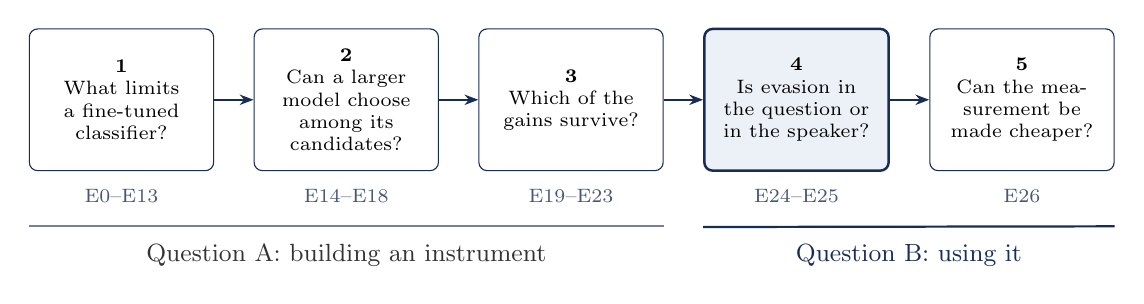
\begin{tikzpicture}[
      font=\scriptsize,
      phase/.style={draw=navy, rounded corners=3pt, align=center, fill=white, text width=22mm, minimum height=18mm, inner sep=2pt},
      good/.style={phase, fill=soft, line width=0.9pt},
      arr/.style={-{Stealth[length=5pt]}, navy, thick},
      lab/.style={font=\scriptsize, text=navy!80}]
    \node[phase] (s1) {\textbf{1}\\ What limits a fine-tuned classifier?};
    \node[phase, right=5mm of s1] (s2) {\textbf{2}\\ Can a larger model choose among its candidates?};
    \node[phase, right=5mm of s2] (s3) {\textbf{3}\\ Which of the gains survive?};
    \node[good, right=5mm of s3] (s4) {\textbf{4}\\ Is evasion in the question or in the speaker?};
    \node[phase, right=5mm of s4] (s5) {\textbf{5}\\ Can the measurement be made cheaper?};
    \foreach \a/\b in {s1/s2,s2/s3,s3/s4,s4/s5} \draw[arr] (\a) -- (\b);
    \foreach \n/\e in {s1/{E0--E13},s2/{E14--E18},s3/{E19--E23},s4/{E24--E25},s5/E26}
      \node[below=1mm of \n, lab] {\e};
    \draw[navy!60, thick] ([yshift=-7mm]s1.south west) -- ([yshift=-7mm]s3.south east)
      node[midway, below=1mm, font=\small, text=black!80] {Question A: building an instrument};
    \draw[navy, thick] ([yshift=-7mm]s4.south west) -- ([yshift=-7mm]s5.south east)
      node[midway, below=1mm, font=\small, text=navy] {Question B: using it};
  \end{tikzpicture}
  \vspace{4pt}
  \begin{itemize}\small\raggedright
    \item Each experiment's plan, prediction and decision rule was written down \emph{before} the run. Results we did not register are marked \explor.
    \item Each result slide shows what we \textbf{predicted} next to what we \textbf{found}, including the many predictions that failed.
    \item Claims rest on 10 paired seeds. Parameters fitted on dev are scored by nested cross-validation, and the one choice made on dev after a failure ($\delta = 0.5$ for the distilled point) is flagged.
    \item From Stage 4 on, one frozen system labels everything, so no parameter changes between experiments.
  \end{itemize}
\end{frame}

% ====================================================================== STAGE 1
\setstage{Stage 1: what limits a classifier?}
\begin{frame}{The classification pipeline shared by both backbones}
  \centering
  \resizebox{\textwidth}{!}{% Figure 1: the classification pipeline (TikZ, monochrome). Input by \FigureArch in figs.tex.
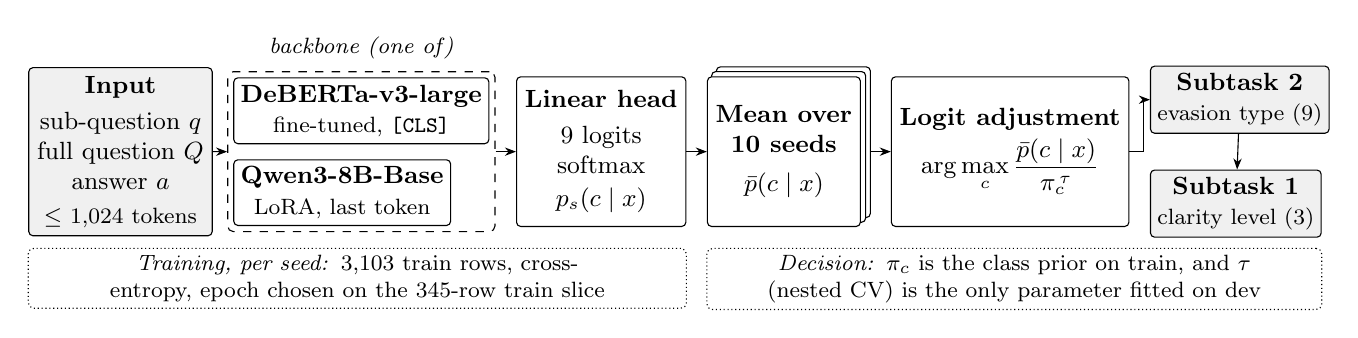
\begin{tikzpicture}[
  font=\small,
  node distance=2.6mm,
  box/.style={draw, rounded corners=1.5pt, align=center, inner xsep=3pt, inner ysep=3pt, minimum height=#1},
  box/.default=19mm,
  sub/.style={draw, rounded corners=1.5pt, align=center, inner sep=2.5pt, minimum width=#1},
  sub/.default=25mm,
  arr/.style={-{Stealth[length=4pt]}, thin},
  note/.style={font=\footnotesize\itshape, align=center},
  band/.style={draw, densely dotted, rounded corners=2pt, inner sep=2.5pt, align=center, font=\footnotesize},
]
% Input
\node[box, fill=black!6] (in) {%
  \textbf{Input}\\[2pt]
  sub-question $q$\\
  full question $Q$\\
  answer $a$\\[1pt]
  {\footnotesize $\le$ 1{,}024 tokens}};

% Backbone: one of two
\node[sub, right=of in, yshift=5.2mm] (deb) {\textbf{DeBERTa-v3-large}\\{\footnotesize fine-tuned, \texttt{[CLS]}}};
\node[sub, right=of in, yshift=-5.2mm] (qwen) {\textbf{Qwen3-8B-Base}\\{\footnotesize LoRA, last token}};
\node[draw, dashed, rounded corners=2pt, inner sep=2pt, fit=(deb)(qwen)] (bb) {};
\node[note, above=0.3mm of bb] {backbone (one of)};

% Head
\node[box, right=of bb] (head) {\textbf{Linear head}\\[2pt] 9 logits\\ softmax\\[1pt] $p_s(c \mid x)$};

% Seed ensemble: stacked outlines stand for the ten trained seeds
\node[box, right=of head, fill=white] (ens) {\textbf{Mean over}\\\textbf{10 seeds}\\[3pt] $\bar p(c \mid x)$};
\begin{scope}[on background layer]
  \draw[rounded corners=1.5pt, fill=white] ($(ens.south west)+(1.2mm,1.2mm)$) rectangle ($(ens.north east)+(1.2mm,1.2mm)$);
  \draw[rounded corners=1.5pt, fill=white] ($(ens.south west)+(0.6mm,0.6mm)$) rectangle ($(ens.north east)+(0.6mm,0.6mm)$);
\end{scope}

% Logit adjustment
\node[box, right=of ens, xshift=1.2mm] (la) {\textbf{Logit adjustment}\\[2pt]
  $\arg\max\limits_c \dfrac{\bar p(c \mid x)}{\pi_c^{\,\tau}}$};

% Outputs
\node[sub=20mm, fill=black!6, right=of la, yshift=6.6mm] (s2) {\textbf{Subtask 2}\\{\footnotesize evasion type (9)}};
\node[sub=20mm, fill=black!6, right=of la, yshift=-6.6mm] (s1) {\textbf{Subtask 1}\\{\footnotesize clarity level (3)}};

% Arrows
\draw[arr] (in) -- (bb);
\draw[arr] (bb) -- (head);
\draw[arr] (head) -- (ens);
\draw[arr] ($(ens.east)+(1.2mm,0)$) -- (la);
\draw[arr] (la.east) -- ++(1.8mm,0) |- (s2.west);
\draw[arr] (s2) -- (s1);

% Training and decision notes
\path let \p1=(in.west), \p2=(head.east), \p3=(bb.south) in
  node[band, anchor=north, text width=\x2-\x1-5pt] at ({(\x1+\x2)/2}, \y3-2mm) (train) {%
  \textit{Training, per seed:} 3{,}103 train rows, cross-entropy, epoch chosen on the 345-row train slice};
\path let \p1=(ens.west), \p2=(s1.east), \p3=(train.north) in
  node[band, anchor=north, text width=\x2-\x1-5pt] at ({(\x1+\x2)/2}, \y3) (dec) {%
  \textit{Decision:} $\pi_c$ is the class prior on train, and $\tau$ (nested CV) is the only parameter fitted on dev};
\end{tikzpicture}
}
  \vspace{6pt}
  \begin{itemize}\small
    \item \textbf{Backbone (one of two):} DeBERTa-v3-large, fully fine-tuned, reads the \texttt{[CLS]} state. Qwen3-8B-Base with LoRA reads the last token. Both see the sub-question $q$, the full question $Q$ and the answer $a$ ($\le$ 1,024 tokens).
    \item \textbf{Head:} a new linear layer gives 9 logits and a softmax $p_s(c\mid x)$ over the evasion types for each seed $s$.
    \item \textbf{System:} average the 10 seeds into $\bar p(c\mid x)$, then divide by the train class prior $\pi_c$ raised to $\tau$.
    \item \textbf{Output:} the Subtask 2 label (9 types) fixes the Subtask 1 clarity level (3) through the taxonomy.
  \end{itemize}
\end{frame}

\begin{frame}{A controlled DeBERTa baseline and seed ensembling}
  \centering
  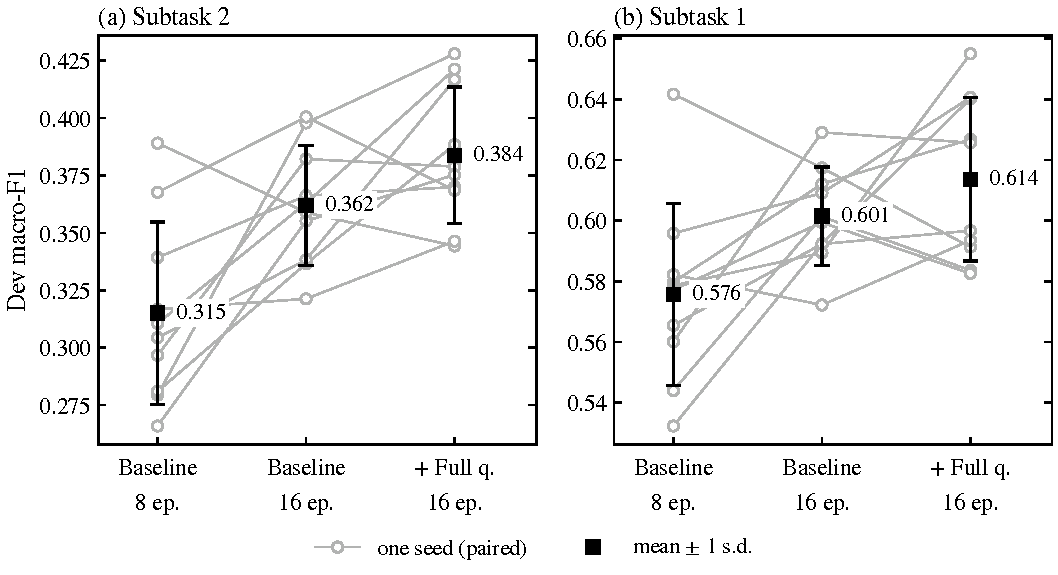
\includegraphics[height=0.43\textheight]{figures/deberta_seeds.pdf}
  \vspace{2pt}
  \begin{itemize}\small
    \item[] \textcolor{navy}{\textbf{Seeds:}} the ten models differ only in their random seed. Averaging their softmax outputs reduces the variance between runs, and every claim in this talk compares paired seeds.
        \item[] \textcolor{navy}{\textbf{Result:}} 16 epochs plus the full question raised the model from \hl{0.315 to 0.384} (+0.069, 9 of 10 seeds up). The 10-seed system with logit adjustment scores 0.405 S2 and 0.648 S1.
    \item[] \textcolor{navy}{\textbf{Takeaway:}} undertraining hid the gain (at 8 epochs, 0.282 against 0.337, with the loss still at 1.3--1.5), so we report fit next to every score.
  \end{itemize}
\end{frame}

\begin{frame}{The decision rule: logit adjustment}
  \begin{columns}[c]
    \begin{column}{0.46\textwidth}
      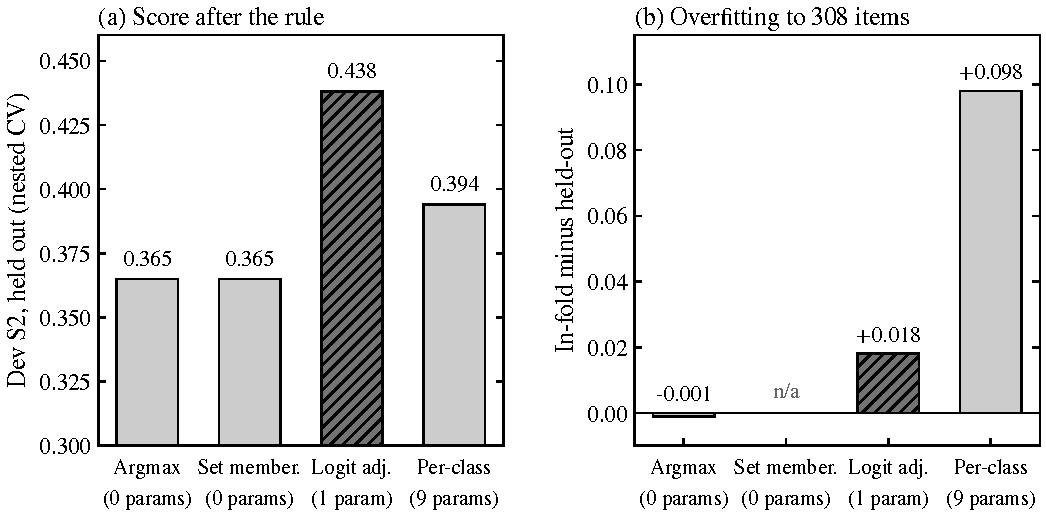
\includegraphics[width=\linewidth]{figures/decision_rules.pdf}
    \end{column}
    \begin{column}{0.52\textwidth}
      \begin{block}{How it works}
        \small
        An argmax picks the class with the highest averaged probability. Macro-F1 weights all nine classes equally, but the train labels are dominated by the Ambivalent types (59\%) and Explicit (31\%).
        Dividing $\bar p(c\mid x)$ by $\pi_c^{\tau}$ lowers the score of frequent classes, so rare ones are predicted more often. With $\tau = 0$ this is the plain argmax, and $\tau = 1$ removes the train prior entirely.
        $\tau$ is the only fitted parameter, chosen on dev by nested cross-validation.
      \end{block}
      \expcard{E4 \quad Logit adjustment against per-class weights}
        {nine free class weights could fit the metric better than one scalar.}
        {logit adjustment 0.365 $\rightarrow$ \hl{0.438}. Nine weights reach only 0.394, with an in-fold gain of +0.098 that does not transfer.}
        {one scalar beats nine weights on 308 items. Every system uses it.}
    \end{column}
  \end{columns}
\end{frame}

\begin{frame}{Structural changes failed, while the decision rule, training length and full question helped}
  \begin{columns}[c]
    \begin{column}{0.44\textwidth}
      \begin{block}{Four explanations for the plateau (DeBERTa-v3-large)}
        \small
        \begin{itemize}\setlength{\itemsep}{2pt}
          \item \textbf{Noisy labels?} No: 53 errors were on items all annotators agreed on.
          \item \textbf{The decision rule?} A little: logit adjustment +0.073.
          \item \textbf{Label meaning?} No: a re-ranker given label definitions $-$0.011, though gold was in the top 3 for 90\%.
          \item \textbf{Missing knowledge?} $\rightarrow$ tested by changing the backbone.
        \end{itemize}
      \end{block}
    \end{column}
    \begin{column}{0.54\textwidth}
      \centering
      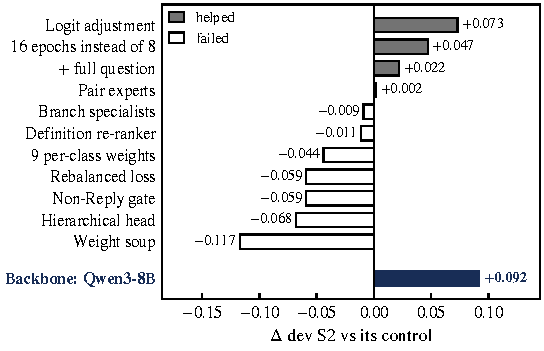
\includegraphics[width=\linewidth,height=0.62\textheight,keepaspectratio]{figures/s_changes.pdf}
    \end{column}
  \end{columns}
  \takeaway{no structural change moved the system, so we changed the model itself.}
\end{frame}

\begin{frame}{Where the DeBERTa ensemble fails}
  \begin{columns}[c]
    \begin{column}{0.5\textwidth}
      \centering
      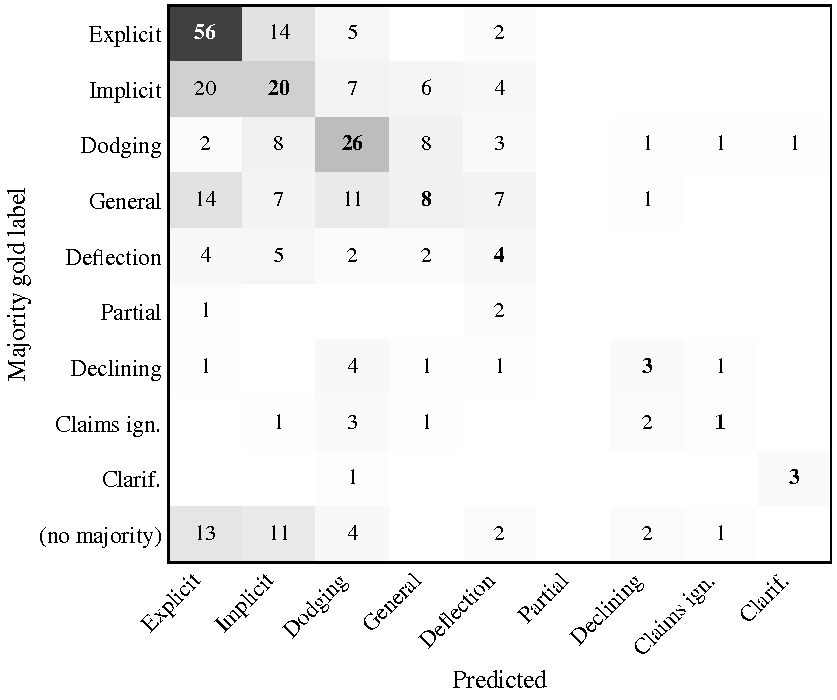
\includegraphics[width=\linewidth,height=0.66\textheight,keepaspectratio]{figures/confusion.pdf}
    \end{column}
    \begin{column}{0.46\textwidth}
      \footnotesize
      \begin{block}{How to read it}
        \footnotesize
        \begin{itemize}
          \item Rows are the majority gold label (at least 2 of 3 annotators), plus a ``no majority'' row (33 items).
          \item Columns are the argmax of the 10-seed ensemble. The diagonal is right for 121 of 275 majority items.
          \item Scoring never uses the majority. A prediction counts if \emph{any} annotator gave it.
        \end{itemize}
      \end{block}
      \begin{block}{What it tells us}
        \footnotesize
        \begin{itemize}
          \item Errors sit inside \emph{Ambivalent}. Implicit is predicted as Explicit 20 times, and General is spread over five other labels.
          \item Partial/half-answer is never predicted.
          \item The encoder fails on \hl{how committed} an answer is, the same pairs annotators disagree on.
        \end{itemize}
      \end{block}
    \end{column}
  \end{columns}
  \takeaway{a model with more knowledge should improve these boundaries. We test this by changing only the backbone.}
\end{frame}

\begin{frame}{A stronger pretrained backbone gained more per model than all encoder changes combined}
  \begin{columns}[c]
    \begin{column}{0.46\textwidth}
      \centering
      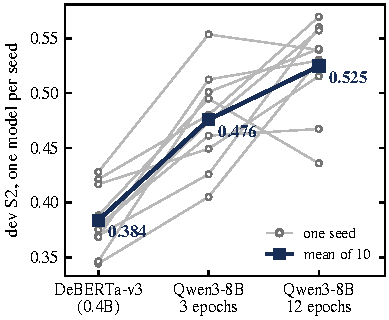
\includegraphics[width=\linewidth,height=0.64\textheight,keepaspectratio]{figures/s_backbone.pdf}
    \end{column}
    \begin{column}{0.52\textwidth}
      \small
      One change: DeBERTa-v3-large $\rightarrow$ Qwen3-8B-Base + LoRA, with the same rows, input, loss and selection, on 10 paired seeds.
      \vspace{4pt}

      \textcolor{navy}{\textbf{Expected:}} gains on the Explicit--Implicit--General boundaries of the confusion matrix\\[3pt]
      \found{+0.092 per model, 10 of 10 seeds up (all encoder changes together: +0.069)}\\[3pt]
      \found{the gain is broad, largest on the Non-Reply types (Claims ignorance +0.40), so the expected location did not hold} \failed
      \vspace{4pt}

      {\footnotesize\textcolor{gray}{``Stronger backbone'', not ``knowledge'' alone: size, pretraining, LoRA and the head all changed together.}}
    \end{column}
  \end{columns}
  \raises{the 8B model ranks the right label far better than it picks it.}
\end{frame}

% ====================================================================== STAGE 2
\setstage{Stage 2: the cascade}
\begin{frame}{The classifier ranks the right label better than it picks it}
  \centering
  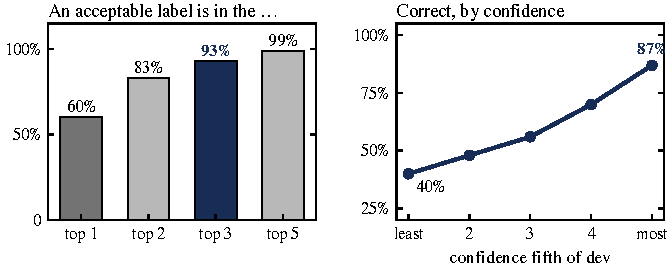
\includegraphics[width=0.92\linewidth,height=0.58\textheight,keepaspectratio]{figures/s_ranking.pdf}
  \par\vspace{4pt}\raggedright
  \takeaway{errors are mostly a choice among a few top candidates, made where the model is unsure. So let a larger model choose among them, \emph{only} for the least confident items.}
\end{frame}

\begin{frame}{System design: a classifier, a router and an LLM adjudicator}
  \centering
  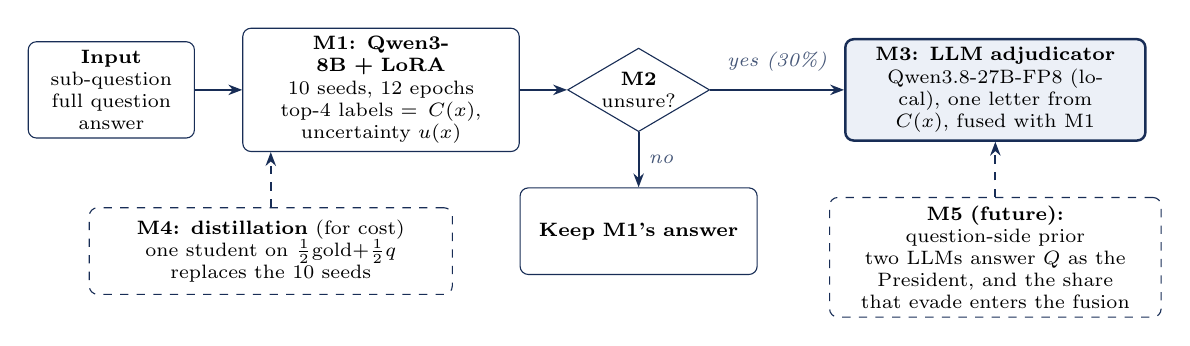
\begin{tikzpicture}[
      font=\scriptsize,
      box/.style={draw=navy, rounded corners=3pt, align=center, fill=white, minimum height=11mm, inner sep=3pt},
      main/.style={box, fill=soft, line width=0.9pt},
      arr/.style={-{Stealth[length=5pt]}, navy, thick},
      lab/.style={font=\scriptsize\itshape, text=navy!80}]
    \node[box, text width=19mm] (in) {\textbf{Input}\\sub-question\\full question\\answer};
    \node[box, text width=33mm, right=6mm of in] (m1) {\textbf{M1: Qwen3-8B + LoRA}\\10 seeds, 12 epochs\\top-4 labels $=C(x)$, uncertainty $u(x)$};
    \node[draw=navy, diamond, aspect=1.7, inner sep=0.5pt, align=center, right=6mm of m1] (m2) {\textbf{M2}\\unsure?};
    \node[main, text width=36mm, right=17mm of m2] (m3) {\textbf{M3: LLM adjudicator}\\Qwen3.8-27B-FP8 (local), one letter from $C(x)$, fused with M1};
    \node[box, text width=28mm, below=7mm of m2] (keep) {\textbf{Keep M1's answer}};
    \node[box, text width=44mm, dashed, below=7mm of m1, xshift=-14mm] (m4) {\textbf{M4: distillation} (for cost)\\one student on $\tfrac12$gold$+\tfrac12 q$ replaces the 10 seeds};
    \node[box, dashed, text width=40mm, below=7mm of m3] (m5) {\textbf{M5 (future):} question-side prior\\two LLMs answer $Q$ as the President, and the share that evade enters the fusion};
    \draw[arr, dashed] (m5.north) -- (m3.south);
    \draw[arr] (in) -- (m1);
    \draw[arr] (m1) -- (m2);
    \draw[arr] (m2) -- node[lab, above, yshift=1mm] {yes (30\%)} (m3);
    \draw[arr] (m2) -- node[lab, right] {no} (keep);
    \draw[arr, dashed] (m4.north) -- (m4.north |- m1.south);
  \end{tikzpicture}
  \vspace{2pt}
  \begin{itemize}\footnotesize\raggedright
    \item Registered checks that set the design: choosing at random inside M1's top 3 \emph{lowers} S2 (0.587 vs 0.598), so the LLM is \hl{fused} with M1, not substituted. Candidate sets by probability mass did not transfer to new rows, but sets by rank did (\textbf{top 4}).
    \item On 300 cross-fitted train rows (fused accuracy), retrieved examples \emph{hurt} the 27B (0.330 vs 0.353 without), and a 304B model did worse than the local 27B (0.317): short prompt, local model, one output token.
  \end{itemize}
\end{frame}

\begin{frame}{Deferral rate against cost on dev}
  \begin{columns}[c]
    \begin{column}{0.50\textwidth}
      \centering
      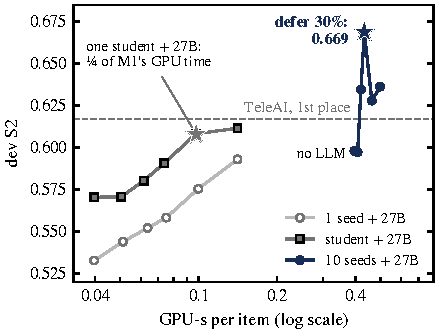
\includegraphics[width=\linewidth,height=0.68\textheight,keepaspectratio]{figures/s_frontier.pdf}
    \end{column}
    \begin{column}{0.48\textwidth}
      \small
      \begin{itemize}\setlength{\itemsep}{3pt}
        \item \textbf{Defer 30\%}: \hl{0.669}, +0.067 over M1 \src{[+0.009, +0.124], parameters held fixed}, with 33 items fixed and 9 broken (after we fixed a bug in our own fusion code).
        \item \textbf{Defer everything}: worse (0.609 over ten splits). Where M1 is confident, the LLM is the weaker reader.
        \item \textbf{Distil}: one student plus the 27B matches the ten-seed M1 at a quarter of its GPU time. Ten students add only +0.005 (ten M1 seeds: +0.065).
      \end{itemize}
    \end{column}
  \end{columns}
  \raises{was 0.669 luck? One ensemble, parameters fitted on 308 items.}
\end{frame}

\setstage{Example: a shared answer}
\begin{frame}{One answer, two sub-questions, two labels}
  \begin{block}{One journalist's turn at a President's news conference, and one answer}
    \small ``Is that a make-or-break issue for you, in terms of domestic politics? There's a Republican in Pennsylvania who says he doesn't think the troops should \ldots\ would you campaign for Mike Fitzpatrick?''
    \par\vspace{3pt}\centering\textcolor{navy}{\large\textbf{``I already have.''}}
  \end{block}
  \begin{columns}[T]
    \begin{column}{0.48\textwidth}
      \excard{Explicit \quad (3 of 3 annotators)}
        {Would you campaign for Mike Fitzpatrick?}
        {I already have.}
        {the answer states what was asked.}
    \end{column}
    \begin{column}{0.48\textwidth}
      \excard{Dodging \quad (3 of 3 annotators)}
        {Is that a make-or-break issue for you, in terms of domestic politics?}
        {I already have.}
        {the answer says nothing about whether the issue is make-or-break.}
    \end{column}
  \end{columns}
  \takeaway{69\% of training rows share their answer with another sub-question, so one answer can receive two labels. Whether an answer evades then depends on the question it is paired with. Stage~4 tests this, and the last slides return to this answer.}
\end{frame}

% ====================================================================== STAGE 3
\setstage{Stage 3: which gains survive?}
\begin{frame}{Controls on the cascade: routing, fusion and where the 27B helps}
  \centering
  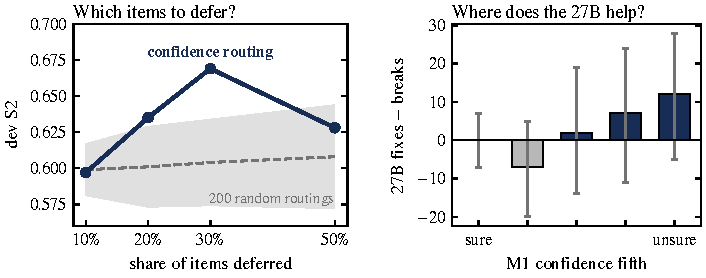
\includegraphics[width=0.96\linewidth,height=0.46\textheight,keepaspectratio]{figures/s_robust.pdf}
  \par\vspace{4pt}\raggedright
  \begin{itemize}\small
    \item On 3,448 cross-fitted train rows the cascade gains +0.014 \src{[+0.002, +0.026]}, less than on dev, where its parameters were fitted.
    \item No random routing of the same size matches confidence routing (0.669 against 0.604 $\pm$ 0.015 over 200 draws). The 27B alone over all nine labels scores 0.591, below M1 (0.598), so fusion is needed.
    \item The 27B fixes about as many items as it breaks where M1 is confident and helps only where M1 is unsure. A learned fix/break router lost to confidence at 4 of 4 budgets.
  \end{itemize}
\end{frame}

\begin{frame}{The 27B prioritises option A}
  \centering
  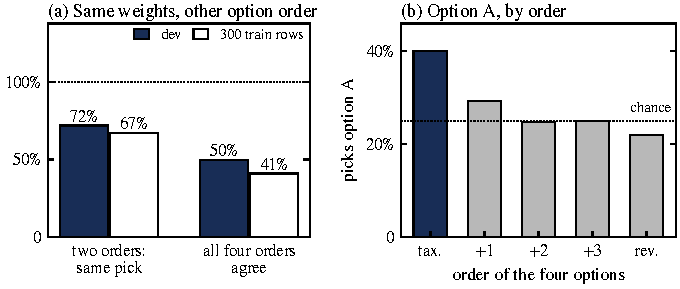
\includegraphics[width=0.96\linewidth,height=0.42\textheight,keepaspectratio]{figures/s_nondet.pdf}
  \par\vspace{3pt}\raggedright
  \begin{itemize}\small
    \item LLMs choosing among lettered options are known to prefer some positions (Zheng et al., ICLR 2024). Ours prioritises \hl{option A}: it picks A for 40\% of items in taxonomy order, against 22--29\% in the other orders (chance is 25\%).
    \item In taxonomy order slot A usually holds Explicit, so a preference for A is also a preference for Explicit.
    \item Two orders of the same four candidates give the same pick on only 72\% of dev items.
    \item We therefore average four cyclic orders. This costs four calls per deferred item and moved the system by +0.011 at split 0 but only +0.002 over ten splits.
  \end{itemize}
  \takeaway{the final system averages four option orders, and all later numbers use that setting.}
  \par{\scriptsize\textcolor{gray}{C.\ Zheng, H.\ Zhou, F.\ Meng, J.\ Zhou, M.\ Huang. Large Language Models Are Not Robust Multiple Choice Selectors. ICLR 2024.}}
\end{frame}

\begin{frame}{The frozen system compared with the winning system}
  \begin{columns}[T]
    \begin{column}{0.60\textwidth}
      \footnotesize
      \setlength{\tabcolsep}{3.5pt}
      \begin{tabular}{@{}lcccc@{}}
        \toprule
        System (dev) & S2 & S1 & LLM calls & GPU-s \\
        \midrule
        DeBERTa-v3-large, 10 seeds & 0.405 & 0.648 & 0 & -- \\
        M1: Qwen3-8B, 10 seeds & 0.598 & 0.743 & 0 & 0.40 \\
        \textbf{Accuracy point}, M1 + 27B & \textbf{0.650} & \textbf{0.788} & 1.43 & 0.54 \\
        \textbf{Distilled point}, 4 orders & \textbf{0.608} & \textbf{0.785} & 2.30 & 0.27 \\
        \quad one option order & 0.599 & 0.784 & 0.57 & 0.10 \\
        \midrule
        TeleAI, 1st place & 0.617 & 0.812 & 1.94 & n/a \\
        \bottomrule
      \end{tabular}
      \vspace{3pt}

      {\scriptsize\textcolor{gray}{Nested-CV split 0 (0.639 over ten splits for the accuracy point). All records re-scored once on one serving setup. LLM calls are 27B calls per item, four per deferred item with four orders. GPU-s is inference time per item, all on one GPU. TeleAI's row is its own dev result, with ${\sim}$7.3k LLM input tokens against our ${\sim}$1.6k. Its GPU time is not published.}}
    \end{column}
    \begin{column}{0.37\textwidth}
      \begin{block}{Relation to the task's system papers}
        \footnotesize
        In the task's 30 system papers, these parts were already in use: candidate sets, LLM choosers, routing, distillation. \textbf{None tested whether such systems read the question.}\\[3pt]
        So we froze every setting and used the cascade as an \hl{instrument}.
      \end{block}
    \end{column}
  \end{columns}
  \raises{if a label is not a property of the answer alone, what is it a property of?}
\end{frame}

% ====================================================================== STAGE 4
\setstage{Stage 4: what it measures}
\begin{frame}{Labels of one answer across its sub-questions}
  \centering
  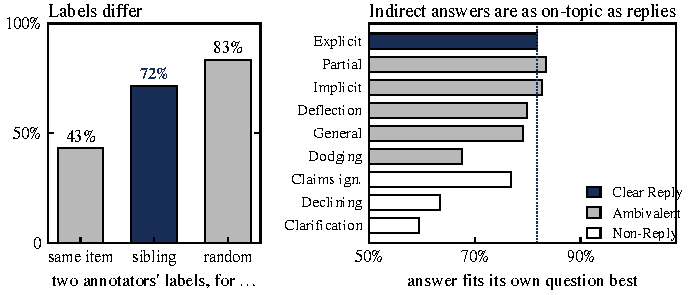
\includegraphics[width=0.94\linewidth,height=0.46\textheight,keepaspectratio]{figures/s_relation.pdf}
  \par\vspace{3pt}\raggedright
  \begin{itemize}\small
    \item On dev, two sub-questions of one answer get different labels 72\% of the time, against 83\% for random items and 43\% for two annotators on the same item. On train, 61.5\% of 3,079 sibling pairs differ.
    \item Partial, Implicit, Deflection and General answers fit their question as well as Explicit ones, so relevance is not answerhood \src{(Clear Reply vs rest: AUROC 0.566)}.
  \end{itemize}
  \takeaway{evasion is a relation between a question and an answer. The ``I already have'' answer is typical, not an exception.}
\end{frame}

\begin{frame}{Validity check: removing or swapping the question}
  \begin{columns}[c]
    \begin{column}{0.40\textwidth}
      \centering
      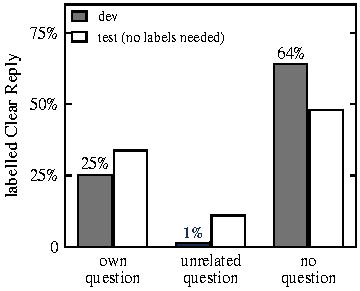
\includegraphics[width=\linewidth,height=0.66\textheight,keepaspectratio]{figures/s_swap.pdf}
    \end{column}
    \begin{column}{0.58\textwidth}
      \small
      A validity check before using it on new speakers: pair each answer with an unrelated question, or with none.\\[4pt]
      \pred{the Clear-Reply share at least halves}\\
      \found{25\% $\rightarrow$ 1\%} \held\\[4pt]
      Surprise: with \emph{no} question, Clear Replies \emph{rise} to 64\%. Without a question, nothing is evaded.
      \vspace{4pt}

      \begin{block}{Our answer again, under an unrelated question}
        \footnotesize
        ``Why did you keep saying there was a relationship between Saddam Hussein, Zarqawi, and Al Qaida \ldots?''\\
        \textcolor{navy}{\textbf{``I already have.''}} $\rightarrow$ instrument: \hl{Dodging}\\
        With its own two questions it gives Explicit and Dodging, as all six annotations say.
      \end{block}
    \end{column}
  \end{columns}
\end{frame}

\begin{frame}{Does the question or the speaker drive evasion? Design}
  \begin{columns}[c]
    \begin{column}{0.52\textwidth}
      \centering
      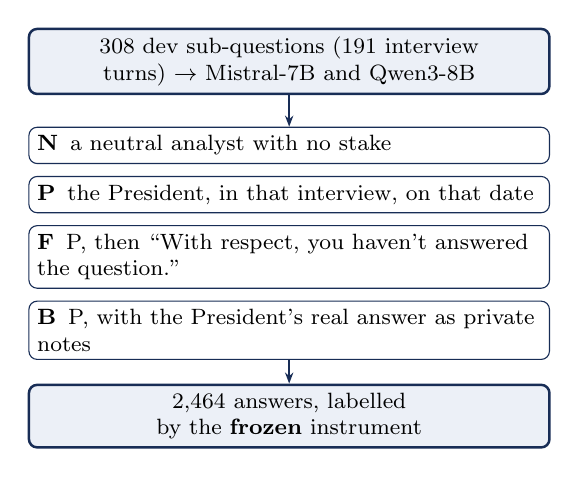
\begin{tikzpicture}[
          font=\footnotesize,
          r/.style={draw=navy, rounded corners=3pt, text width=64mm, align=left, inner sep=3pt, fill=white},
          top/.style={draw=navy, rounded corners=3pt, text width=64mm, align=center, inner sep=3pt, fill=soft, line width=0.9pt},
          arr/.style={-{Stealth[length=4pt]}, navy, thick}]
        \node[top] (q) {308 dev sub-questions (191 interview turns) $\rightarrow$ Mistral-7B and Qwen3-8B};
        \node[r, below=4mm of q] (n) {\textbf{N}\enspace a neutral analyst with no stake};
        \node[r, below=1.5mm of n] (p) {\textbf{P}\enspace the President, in that interview, on that date};
        \node[r, below=1.5mm of p] (f) {\textbf{F}\enspace P, then ``With respect, you haven't answered the question.''};
        \node[r, below=1.5mm of f] (b) {\textbf{B}\enspace P, with the President's real answer as private notes};
        \node[top, below=3mm of b] (o) {2,464 answers, labelled by the \textbf{frozen} instrument};
        \draw[arr] (q) -- (n); \draw[arr] (b) -- (o);
      \end{tikzpicture}
    \end{column}
    \begin{column}{0.45\textwidth}
      \begin{block}{Registered predictions}
        \small
        \begin{itemize}\setlength{\itemsep}{2pt}
          \item If the \textbf{question} drives evasion, a speaker with no stake (N) evades where the Presidents did: odds ratio $\ge 1.5$.
          \item If the \textbf{stake} drives it, playing the President (P) raises the evasion rate by $\ge 0.10$.
          \item \textbf{Pursuit} (F) turns $\ge 50\%$ of evasions into replies.
          \item \textbf{Notes} (B) help more on questions answered indirectly than on non-answers ($\ge +0.15$).
        \end{itemize}
      \end{block}
    \end{column}
  \end{columns}
\end{frame}

\begin{frame}{Evasion rates by role}
  \centering
  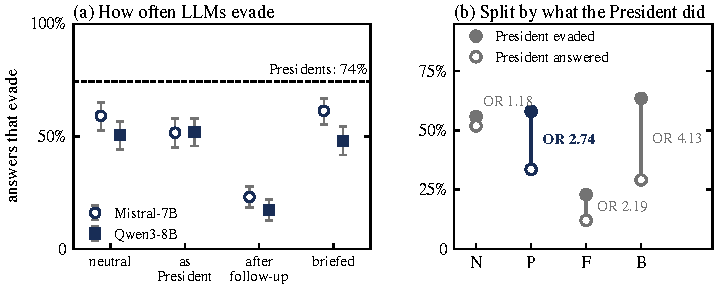
\includegraphics[width=0.93\linewidth,height=0.47\textheight,keepaspectratio]{figures/s_audit.pdf}
  \par\vspace{2pt}
  \begin{columns}[T]
    \begin{column}{0.49\textwidth}
      \footnotesize
      \textbf{No stake (N)}: odds ratio 1.18 \src{[0.80, 1.73]} \failed\\[2pt]
      \textbf{Stake} raises the rate: $-$0.031 \failed\\[2pt]
      \textbf{President's role (P)}: odds ratio \hl{2.74} \src{[1.87, 4.17]} \explor
    \end{column}
    \begin{column}{0.49\textwidth}
      \footnotesize
      \textbf{Pursuit (F)}: 66\% of evasions become replies \held\\[2pt]
      \textbf{Notes (B)}: +0.113 \src{[$-$0.006, +0.225]}, below the bar \failed
    \end{column}
  \end{columns}
  \par\vspace{3pt}
  \small\textcolor{navy}{\textbf{In panel (b)}}, the change is in the open dots. Where the President answered, a neutral analyst still evades 52\%, but in the President's role the models evade only 34\%.
\end{frame}

\begin{frame}{What the role result shows and does not show}
  \begin{columns}[T]
    \begin{column}{0.48\textwidth}
      \begin{block}{What it shows}
        \small
        \begin{itemize}\setlength{\itemsep}{2pt}
          \item The role changes \emph{where} models evade, not \emph{how often} (52\% vs 55\%).
          \item In the President's role they answer directly what the Presidents answered directly. A neutral analyst, to whom the questions are not addressed, evades about half of them whatever the President did.
          \item So a question's answerability shows only for a speaker who can answer it.
          \item It holds for each model separately (Mistral 3.0, Qwen 2.5).
        \end{itemize}
      \end{block}
    \end{column}
    \begin{column}{0.48\textwidth}
      \begin{block}{What it does not show}
        \small
        \begin{itemize}\setlength{\itemsep}{2pt}
          \item It is exploratory, with two model families, one of them the judge's own (Qwen). Our data cannot separate answerability from strategic evasion.
          \item The P prompt adds identity, date and context, not only a stake, and the role odds ratio was not adjusted for answer length.
          \item The instrument was not human-validated on LLM text, though it is \emph{more} confident there (seed agreement 0.81 vs 0.73).
          \item Anything about real politicians' intent.
        \end{itemize}
      \end{block}
    \end{column}
  \end{columns}
  
\end{frame}

\begin{frame}{What the evasion study tells us to act on}
  \small
  Everything so far comes from one pipeline: the classifier, the router, the 27B adjudicator, frozen as an instrument. Its results point to three things to act on.
  \vspace{4pt}

  \begin{columns}[T]
    \begin{column}{0.32\textwidth}
      \begin{block}{1\quad Labels follow the question}
        \footnotesize
        One answer gets different labels under different sub-questions, and the instrument reads the question causally.\\[3pt]
        \textcolor{navy}{\textbf{Act on it:}} always feed the full question with the answer. Never label an answer alone.
      \end{block}
    \end{column}
    \begin{column}{0.32\textwidth}
      \begin{block}{2\quad The question carries signal}
        \footnotesize
        LLMs in the President's role, who never saw the real answer, answer directly the questions the Presidents answered directly (odds ratio 2.74).\\[3pt]
        \textcolor{navy}{\textbf{Act on it:}} no module uses this signal yet. A \hl{question-side prior, M5}, could feed it to the fusion.
      \end{block}
    \end{column}
    \begin{column}{0.32\textwidth}
      \begin{block}{3\quad No shortcut}
        \footnotesize
        Half an answer agrees with the full-answer label on only 66\% of items, and probes on the frozen model reach 0.397 S2 against 0.525 for one fine-tuned seed.\\[3pt]
        \textcolor{navy}{\textbf{Act on it:}} keep the full model and make it cheaper instead. That is Stage 5.
      \end{block}
    \end{column}
  \end{columns}
  \takeaway{the second point gives the next architectural element, M5, to which we return after Stage 5.}
  \raises{can the full instrument run cheaper?}
\end{frame}

% ====================================================================== STAGE 5
\setstage{Stage 5: cheaper?}
\begin{frame}{Cost of reduced precision: memory, throughput and latency}
  \begin{columns}[c]
    \begin{column}{0.60\textwidth}
      \small
      \renewcommand{\arraystretch}{1.3}
      \begin{tabular}{@{}lcc@{}}
        \toprule
        M1, 16-bit $\rightarrow$ reduced & FP8 & NF4 \\
        \midrule
        Throughput (items/s) & 43.1 $\rightarrow$ 35.9 & 7.7 $\rightarrow$ 6.3 \\
        \quad ratio & \hl{0.83$\times$} & \hl{0.82$\times$} \\
        Batch-1 latency, p50 (ms) & 33.6 $\rightarrow$ 30.2 & 169 $\rightarrow$ 259 \\
        \quad ratio & 0.90$\times$ & \hl{1.53$\times$} \\
        Peak memory (GB) & 21.9 $\rightarrow$ 20.9 & 16.8 $\rightarrow$ 11.3 \\
        \quad ratio & \hl{0.96$\times$} & \hl{0.67$\times$} \\
        Label agreement (10 seeds) & 96.1\% & 86.7\% \\
        \bottomrule
      \end{tabular}
      \vspace{3pt}

      {\scriptsize\textcolor{gray}{FP8: native FP8 tensor cores of one RTX PRO 6000 (Blackwell), batch 32 for both. NF4: two RTX A4000, with 16-bit split over two cards at batch 8 and NF4 on one card at batch 16, so its speed is not like for like. Peak memory is per process. The weights of an 8B model alone take about 16, 8 and 4.5\,GB in 16-bit, FP8 and NF4.}}
    \end{column}
    \begin{column}{0.37\textwidth}
      \begin{block}{What we saw}
        \footnotesize
        \begin{itemize}\setlength{\itemsep}{2pt}
          \item \textbf{FP8} ran on native FP8 tensor cores but was slower, not 1.3$\times$ faster as predicted, and barely smaller. Activations are quantized in unfused operations around each matrix product. Reported FP8 speed-ups rely on fused kernels, which we did not use.
          \item \textbf{NF4} saves memory (0.67$\times$, short of the predicted 0.4$\times$) but is slower. Its 4-bit weights are computed in bf16.
          \item Applied to the accuracy point's one-GPU cost, FP8's speed would raise it from 0.538 to 0.619 GPU-s per item (\hl{+15\%}).
        \end{itemize}
      \end{block}
    \end{column}
  \end{columns}
\end{frame}

\begin{frame}{Lower precision: accuracy lost and flipped decisions}
  \centering
  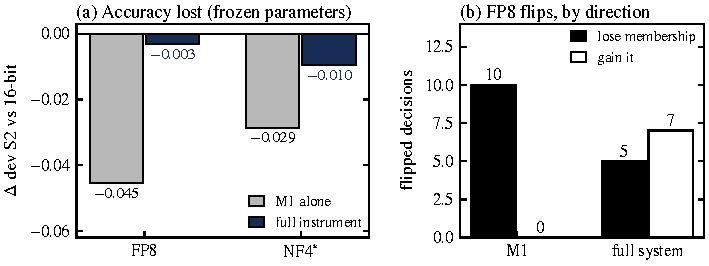
\includegraphics[width=0.93\linewidth,height=0.43\textheight,keepaspectratio]{figures/s_precision.pdf}
  \par\vspace{2pt}\raggedright\footnotesize
  \begin{itemize}\setlength{\itemsep}{1pt}
    \item Frozen M1 in FP8 or NF4, each against 16-bit on the same GPU type. FP8: agreement 96.1\% (bar 98\%) \failed\quad speed 0.83$\times$ (bar 1.3$\times$) \failed\quad flips fall where the 27B re-decides, 71\% vs 36\% by chance \held
    \item All 10 of M1's membership-changing flips lose it, while the system's go both ways (5 lose, 7 gain), so with the same frozen parameters it loses 0.003 against M1's 0.045.
    \item$^{*}$NF4: 27B records are missing for 60 of 136 deferred items and the system flips more decisions than M1 (57 vs 45): no conclusion.
  \end{itemize}
  \takeaway{precision is not a cost lever with these kernels.}
\end{frame}

% ====================================================================== CLOSE
\setstage{Conclusions}
\begin{frame}{Registered predictions that steered the work}
  \footnotesize
  \renewcommand{\arraystretch}{1.7}
  \begin{tabular}{@{}>{\raggedright\arraybackslash}p{0.17\textwidth}>{\raggedright\arraybackslash}p{0.79\textwidth}@{}}
    \textbf{\textcolor{navy}{1\, Classifier}} & \fc{gain on the expected boundaries} \fc{gain larger on agreed items} \\
    \textbf{\textcolor{navy}{2\, Cascade}} & \hc{top-3 headroom} \hc{dev gain at 30\%} \fc{5 seeds $\approx$ 10} \fc{examples help} \fc{student at 30\%} \fc{student ranks errors better} \\
    \textbf{\textcolor{navy}{3\, What survives}} & \hc{test text matters} \fc{learned router} \fc{LLM-knowledge distillation} \fc{cached prompt} \fc{escalation ladder} \\
    \textbf{\textcolor{navy}{4\, What it measures}} & \hc{reads the question} \hc{pursuit} \hc{probe less question-bound} \fc{question-driven (N)} \fc{stake raises rate} \fc{notes} \fc{half answer suffices} \fc{frozen probe suffices} \\
    \textbf{\textcolor{navy}{5\, Precision}} & \hc{FP8 flips land where the 27B re-decides} \fc{FP8 fidelity} \fc{FP8 speed} \fc{NF4 memory (0.4$\times$)} \\
  \end{tabular}
  \vspace{4pt}

  \small
  \hc{held}~registered prediction held \qquad \fc{failed}~failed, and changed the next step\\[2pt]
  {\footnotesize\textcolor{gray}{A selection of the registered predictions that steered the work. Every one, held or not, is in the experiment log.}}
\end{frame}

\begin{frame}{Limitations, each with what we did and what comes next}
  \small
  \renewcommand{\arraystretch}{1.2}
  \begin{tabular}{@{}>{\raggedright\arraybackslash}p{0.27\textwidth}>{\raggedright\arraybackslash}p{0.30\textwidth}>{\raggedright\arraybackslash}p{0.37\textwidth}@{}}
    \toprule
    \textbf{Limitation} & \textbf{What we did} & \textbf{Next step} \\
    \midrule
    308 dev items, and test labels unreleased & 10 paired seeds and nested CV & Score the frozen test predictions once labels are out, and test a second corpus \\
    Not human-checked on LLM text & Label-free check: more confident on LLM text & Two annotators, 100 answers, the registered agreement bar \\
    Two LLM families, and the role effect is exploratory & Per-model results & Add Llama and OLMo, register the role effect and adjust it for answer length \\
    LLM decisions depend on option order and the serving stack & Four orders averaged, one serving setup & Repeat runs (none yet) and pin software and hardware \\
    Quantization not faster as implemented & Same GPU type, and the same batch for FP8 & Fused FP8 kernels, QLoRA for NF4, and every NF4-deferred item scored \\
    \bottomrule
  \end{tabular}
\end{frame}

\begin{frame}{Future work: a question-side evasion prior}
  \begin{columns}[T]
    \begin{column}{0.52\textwidth}
      \begin{block}{Proposed module M5}
        \footnotesize
        \begin{itemize}\setlength{\itemsep}{2pt}
          \item Every module reads the answer, but the role study suggests the question carries evasion signal of its own.
          \item For the items M2 defers, two open LLMs answer the question as the President, \emph{without} the real answer.
          \item The frozen instrument labels those answers, and the share that evade enters the fusion as an extra term.
          \item Its weight is fitted on training rows, whose P-role answers must still be generated. The prediction will be registered before dev is scored.
        \end{itemize}
      \end{block}
    \end{column}
    \begin{column}{0.44\textwidth}
      \begin{block}{Preliminary check on dev \explor}
        \footnotesize
        \renewcommand{\arraystretch}{1.15}
        \begin{tabular}{@{}cccc@{}}
          \toprule
          P-role LLMs & & & President \\
          that evade & items & & evaded \\
          \midrule
          0 of 2 & 101 & & 61\% \\
          1 of 2 & 95 & & 72\% \\
          2 of 2 & 112 & & \hl{88\%} \\
          \bottomrule
        \end{tabular}
        \vspace{3pt}

        Added to M1 it helps only a little. AUROC for ``the President evaded'' goes from 0.872 to 0.875 on all items and from 0.722 to 0.746 on the 111 items M1 is least sure of.
      \end{block}
    \end{column}
  \end{columns}
  \vspace{2pt}
  {\small\textcolor{navy}{\textbf{Expected effect:}} a small gain on the items M1 is unsure about, mainly on the evade-or-not decision. It costs two extra generations per deferred item and needs the instrument to be valid on LLM text.}
  \par\vspace{2pt}{\tiny\textcolor{gray}{The check was written after the E25 results, on 308 dev items. It motivates a registered test and is not evidence for the module.}}
\end{frame}

\begin{frame}{Conclusions}
  \begin{columns}[T]
    \begin{column}{0.58\textwidth}
      \begin{block}{What we learned}
        \small
        \begin{enumerate}\setlength{\itemsep}{4pt}
          \item \textbf{A stronger pretrained backbone, not more structure,} broke the classifier plateau, with +0.092 per model on 10 of 10 seeds.
          \item \textbf{Rank, then adjudicate only where unsure.} The cascade reaches 0.65 dev S2, on par with the winner, with three quarters of its LLM calls. A distilled variant needs a quarter of the classifier's GPU time.
          \item \textbf{Evasion is a relation.} Labels follow the question. In two LLMs, in the President's role, models answer directly what the Presidents answered directly (exploratory). This motivates M5, a question-side prior.
        \end{enumerate}
      \end{block}
    \end{column}
    \begin{column}{0.38\textwidth}
      \begin{block}{The shared answer, again}
        \small
        \textcolor{navy}{\textbf{``I already have.''}}\\[3pt]
        campaign for him? $\rightarrow$ Explicit\\
        make-or-break? $\rightarrow$ Dodging\\
        an unrelated question? $\rightarrow$ Dodging\\[3pt]
        {\footnotesize The instrument gets all three, because it reads the pair.}
      \end{block}
    \end{column}
  \end{columns}
\end{frame}

\begin{frame}{Thank you. Questions?}
  \vspace{6mm}
  \centering
  \begin{block}{Code, pre-registered log and every raw output}
    \centering\small\texttt{github.com/IamSid44/CLARITY-Unmasking-Political-Question-Evasions}
  \end{block}
  \vspace{2mm}
  \small
  \textcolor{navy}{\textbf{Runs and adapters}}\enspace\texttt{huggingface.co/siddarthg44/clarity-semeval26}\\[3pt]
  \textcolor{navy}{\textbf{Training curves}}\enspace\texttt{wandb.ai/iamsid44-iiit-hyderabad/clarity-semeval26}
\end{frame}


\end{document}
